
\documentclass[border=8pt, multi, tikz]{standalone}
\usepackage{import}
\subimport{layers/}{init}
\usetikzlibrary{positioning}
\usetikzlibrary{3d} %for including external image

\def\ConvColor{rgb:yellow,5;red,2.5;white,5}
\def\GatedConvColor{rgb:yellow,1;red,2.5;white,5}
\def\AtrousColor{rgb:red,1;blue,2.5;white,5}
\def\AttentionColor{rgb:orange,5;red,5}
% \def\PoolColor{rgb:red,1;black,0.3}
% \def\UnpoolColor{rgb:blue,2;green,1;black,0.3}
% \def\FcColor{rgb:blue,5;red,2.5;white,5}
% \def\FcReluColor{rgb:blue,5;red,5;white,4}
% \def\SoftmaxColor{rgb:magenta,5;black,7}
% \def\SumColor{rgb:blue,5;green,15}

\newcommand{\copymidarrow}{\tikz \draw[-Stealth,line width=0.8mm,draw={rgb:blue,4;red,1;green,1;black,3}] (-0.3,0) -- ++(0.3,0);}

\begin{document}
\begin{tikzpicture}
\tikzstyle{connection}=[ultra thick,every node/.style={sloped,allow upside down},draw=\edgecolor,opacity=0.7]
\tikzstyle{copyconnection}=[ultra thick,every node/.style={sloped,allow upside down},draw={rgb:blue,4;red,1;green,1;black,3},opacity=0.7]

\node[canvas is zy plane at x=0] (temp) at (-1.5,0,0) {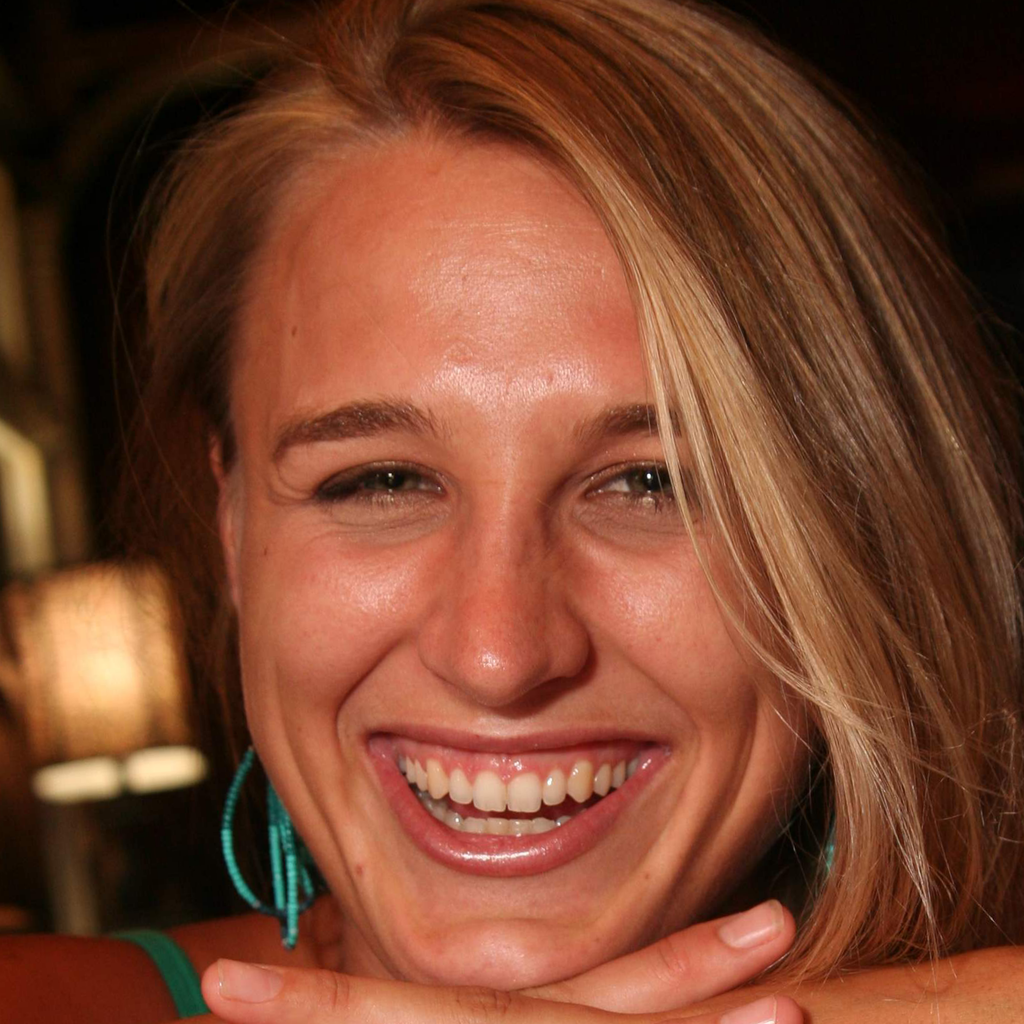
\includegraphics[width=7cm,height=7cm]{input.png}};


\pic[shift={ (0,0,0) }] at (0,0,0)
    {Box={
        name=gate1,
        caption= ,
        % xlabel=,
        % zlabel=32,
        fill=\GatedConvColor,
        % bandfill=\ConvReluColor,
        height=32,
        depth=32,
        width=2
        }
    };

\draw [connection]  ({-1.5,0,0})    -- node {\midarrow} (gate1-east);

\pic[shift={ (0,0,0) }] at (gate1-east)
    {Box={
        name=gate2,
        caption= ,
        % xlabel=128,
        % zlabel=64,
        fill=\GatedConvColor,
        opacity=0.5,
        height=16,
        depth=16,
        width=4
        }
    };

\pic[shift={ (0,0,0) }] at (gate2-east)
    {Box={
        name=gate3,
        caption= ,
        % xlabel=128,
        % zlabel=64,
        fill=\GatedConvColor,
        opacity=0.5,
        height=16,
        depth=16,
        width=4
        }
    };

\pic[shift={ (0,0,0) }] at (gate3-east)
    {Box={
        name=gate4,
        caption= ,
        % xlabel=128,
        % zlabel=64,
        fill=\GatedConvColor,
        opacity=0.5,
        height=8,
        depth=8,
        width=8
        }
    };

\pic[shift={ (0,0,0) }] at (gate4-east)
    {Box={
        name=gate5,
        caption= ,
        % xlabel=128,
        % zlabel=64,
        fill=\GatedConvColor,
        opacity=0.5,
        height=8,
        depth=8,
        width=8
        }
    };

\pic[shift={ (0,0,0) }] at (gate5-east)
    {Box={
        name=gate6,
        caption= ,
        % xlabel=128,
        % zlabel=64,
        fill=\GatedConvColor,
        opacity=0.5,
        height=8,
        depth=8,
        width=8
        }
    };

\pic[shift={ (0,0,0) }] at (gate5-east)
    {Box={
        name=atrous1,
        caption= ,
        % xlabel=128,
        % zlabel=64,
        fill=\AtrousColor,
        opacity=0.5,
        height=8,
        depth=8,
        width=8
        }
    };

\pic[shift={ (0,0,0) }] at (atrous1-east)
    {Box={
        name=atrous2,
        caption= ,
        % xlabel=128,
        % zlabel=64,
        fill=\AtrousColor,
        opacity=0.5,
        height=8,
        depth=8,
        width=8
        }
    };

\pic[shift={ (0,0,0) }] at (atrous2-east)
    {Box={
        name=atrous3,
        caption= ,
        % xlabel=128,
        % zlabel=64,
        fill=\AtrousColor,
        opacity=0.5,
        height=8,
        depth=8,
        width=8
        }
    };

\pic[shift={ (0,0,0) }] at (atrous3-east)
    {Box={
        name=atrous4,
        caption= ,
        % xlabel=128,
        % zlabel=64,
        fill=\AtrousColor,
        opacity=0.5,
        height=8,
        depth=8,
        width=8
        }
    };

\pic[shift={ (0,0,0) }] at (atrous4-east)
    {Box={
        name=gate6,
        caption= ,
        % xlabel=128,
        % zlabel=64,
        fill=\GatedConvColor,
        opacity=0.5,
        height=8,
        depth=8,
        width=8
        }
    };

\pic[shift={ (0,0,0) }] at (gate6-east)
    {Box={
        name=gate7,
        caption= ,
        % xlabel=128,
        % zlabel=64,
        fill=\GatedConvColor,
        opacity=0.5,
        height=8,
        depth=8,
        width=8
        }
    };

\pic[shift={ (0,0,0) }] at (gate7-east)
    {Box={
        name=gate8,
        caption= ,
        % xlabel=128,
        % zlabel=64,
        fill=\GatedConvColor,
        opacity=0.5,
        height=16,
        depth=16,
        width=4
        }
    };

\pic[shift={ (0,0,0) }] at (gate8-east)
    {Box={
        name=gate9,
        caption= ,
        % xlabel=128,
        % zlabel=64,
        fill=\GatedConvColor,
        opacity=0.5,
        height=16,
        depth=16,
        width=4
        }
    };

\pic[shift={ (0,0,0) }] at (gate9-east)
    {Box={
        name=gate10,
        caption= ,
        % xlabel=128,
        % zlabel=64,
        fill=\GatedConvColor,
        opacity=0.5,
        height=32,
        depth=32,
        width=2
        }
    };

\draw [connection]  (gate10-west)    -- node {\midarrow} ({19,0,0});

\node[canvas is zy plane at x=3, shift={(0,0,0)}] (0,0,0) at (gate10-west) {
  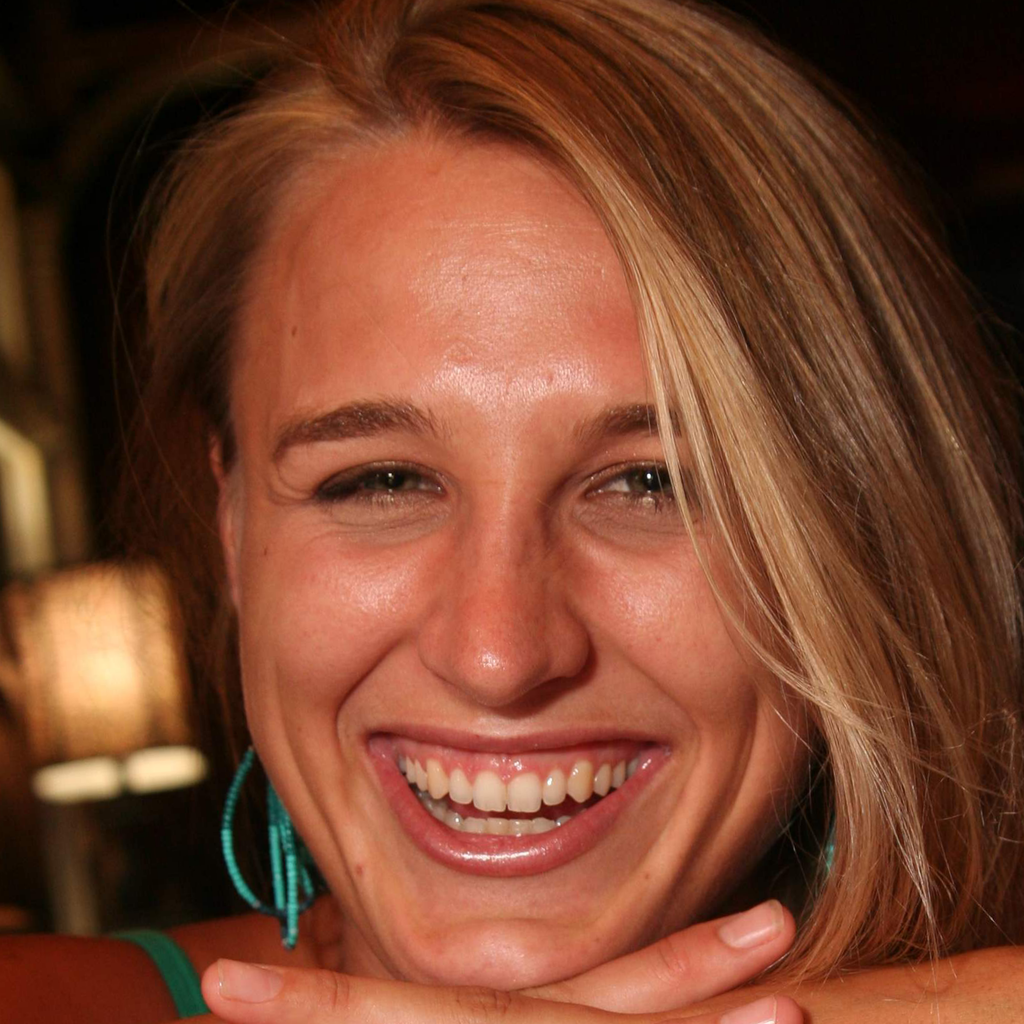
\includegraphics[width=7cm,height=7cm]{input.png}
};

\pic[shift={ (0,-10,0) }] at (0,0,0)
    {Box={
        name=refine1,
        caption= ,
        % xlabel=,
        % zlabel=32,
        fill=\ConvColor,
        % bandfill=\ConvReluColor,
        height=32,
        depth=32,
        width=2
        }
    };

\pic[shift={ (0,0,0) }] at (refine1-east)
    {Box={
        name=refine2,
        caption= ,
        % xlabel=,
        % zlabel=32,
        fill=\ConvColor,
        % bandfill=\ConvReluColor,
        height=21,
        depth=21,
        width=3
        }
    };

\pic[shift={ (0,0,0) }] at (refine2-east)
    {Box={
        name=refine3,
        caption= ,
        % xlabel=,
        % zlabel=32,
        fill=\ConvColor,
        % bandfill=\ConvReluColor,
        height=13,
        depth=13,
        width=5
        }
    };

\pic[shift={ (0,0,0) }] at (refine3-east)
    {Box={
        name=refine4,
        caption= ,
        % xlabel=,
        % zlabel=32,
        fill=\ConvColor,
        % bandfill=\ConvReluColor,
        height=8,
        depth=8,
        width=8
        }
    };

\pic[shift={ (0,0,0) }] at (refine4-east)
    {Box={
        name=refine5,
        caption= ,
        % xlabel=,
        % zlabel=32,
        fill=\ConvColor,
        % bandfill=\ConvReluColor,
        height=5,
        depth=5,
        width=10
        }
    };

\pic[shift={ (0,0,0) }] at (refine5-east)
    {Box={
        name=refine6,
        caption= ,
        % xlabel=,
        % zlabel=32,
        fill=\ConvColor,
        % bandfill=\ConvReluColor,
        height=5,
        depth=5,
        width=10
        }
    };

\pic[shift={ (0,0,0) }] at (refine6-east)
    {Box={
        name=refine7,
        caption= ,
        % xlabel=,
        % zlabel=32,
        fill=\ConvColor,
        % bandfill=\ConvReluColor,
        height=5,
        depth=5,
        width=10
        }
    };

\pic[shift={ (0,0,0) }] at (refine7-east)
    {Box={
        name=refine8,
        caption= ,
        % xlabel=,
        % zlabel=32,
        fill=\ConvColor,
        % bandfill=\ConvReluColor,
        height=5,
        depth=5,
        width=10
        }
    };

\pic[shift={ (0,0,0) }] at (refine8-east)
    {Box={
        name=refine9,
        caption= ,
        % xlabel=,
        % zlabel=32,
        fill=\AttentionColor,
        % bandfill=\ConvReluColor,
        height=5,
        depth=5,
        width=10
        }
    };

\pic[shift={ (0,0,0) }] at (refine9-east)
    {Box={
        name=refine10,
        caption= ,
        % xlabel=,
        % zlabel=32,
        fill=\ConvColor,
        % bandfill=\ConvReluColor,
        height=5,
        depth=5,
        width=10
        }
    };

\pic[shift={ (0,0,0) }] at (refine10-east)
    {Box={
        name=refine11,
        caption= ,
        % xlabel=,
        % zlabel=32,
        fill=\ConvColor,
        % bandfill=\ConvReluColor,
        height=5,
        depth=5,
        width=10
        }
    };

\pic[shift={ (0,0,0) }] at (refine11-east)
    {Box={
        name=refine12,
        caption= ,
        % xlabel=,
        % zlabel=32,
        fill=\ConvColor,
        % bandfill=\ConvReluColor,
        height=5,
        depth=5,
        width=10
        }
    };

\pic[shift={ (0,0,0) }] at (refine12-east)
    {Box={
        name=refine13,
        caption= ,
        % xlabel=,
        % zlabel=32,
        fill=\ConvColor,
        % bandfill=\ConvReluColor,
        height=8,
        depth=8,
        width=8
        }
    };

\pic[shift={ (0,0,0) }] at (refine13-east)
    {Box={
        name=refine14,
        caption= ,
        % xlabel=,
        % zlabel=32,
        fill=\ConvColor,
        % bandfill=\ConvReluColor,
        height=13,
        depth=13,
        width=5
        }
    };

\pic[shift={ (0,0,0) }] at (refine14-east)
    {Box={
        name=refine15,
        caption= ,
        % xlabel=,
        % zlabel=32,
        fill=\ConvColor,
        % bandfill=\ConvReluColor,
        height=21,
        depth=21,
        width=3
        }
    };

\pic[shift={ (0,0,0) }] at (refine15-east)
    {Box={
        name=refine16,
        caption= ,
        % xlabel=,
        % zlabel=32,
        fill=\ConvColor,
        % bandfill=\ConvReluColor,
        height=32,
        depth=32,
        width=2
        }
    };

% MSSA

\pic[shift={ (3,0,0) }] at (refine4-bottom)
    {Box={
        name=mssa1_1,
        caption= ,
        % xlabel=,
        % zlabel=32,
        fill=\ConvColor,
        % bandfill=\ConvReluColor,
        height=8,
        depth=8,
        width=5
        }
    };

\pic[shift={ (9,0,0) }] at (refine4-bottom)
    {Box={
        name=mssa1_2,
        caption= ,
        % xlabel=,
        % zlabel=32,
        fill=\AttentionColor,
        % bandfill=\ConvReluColor,
        height=8,
        depth=8,
        width=5
        }
    };

\pic[shift={ (4,0,0) }] at (refine3-bottom)
    {Box={
        name=mssa2_1,
        caption= ,
        % xlabel=,
        % zlabel=32,
        fill=\ConvColor,
        % bandfill=\ConvReluColor,
        height=13,
        depth=13,
        width=3
        }
    };

\pic[shift={ (10,0,0) }] at (refine3-bottom)
    {Box={
        name=mssa2_2,
        caption= ,
        % xlabel=,
        % zlabel=32,
        fill=\AttentionColor,
        % bandfill=\ConvReluColor,
        height=13,
        depth=13,
        width=3
        }
    };

\draw [connection]  (refine4-south)    -- node {\midarrow} (refine4-bottom)
                    (refine4-bottom)   -- node {\midarrow} (mssa1_1-west);

\draw [connection]  (mssa1_1-east)    -- node {\midarrow} (mssa1_2-west);

\draw [connection]  (mssa1_2-east)    -- node {\midarrow} (refine13-bottom)
                    (refine13-bottom) -- node {\midarrow} (refine13-south);

\draw [connection]  (refine3-south)    -- node {\midarrow} (refine3-bottom)
                    (refine3-bottom)   -- node {\midarrow} (mssa2_1-west);

\draw [connection]  (mssa2_1-east)    -- node {\midarrow} (mssa2_2-west);

\draw [connection]  (mssa2_2-east)    -- node {\midarrow} (refine14-bottom)
                    (refine14-bottom) -- node {\midarrow} (refine14-south);

\end{tikzpicture}
\end{document}

